\subsection{Autenticação Baseada em Sessão}

Uma sessão web é uma troca de informações semipermanente entre um cliente e um servidor web 
\cite{CALZAVARA2017}. O mecanismo de gerenciamento de estados para o HTTP, baseado em sessões, foi 
especificado na RFC 2109 \cite{RFC2109} com sua versão mais atual especificada na RFC 6265 
\cite{RFC6265}. Este mecanismo utiliza o termo \emph{cookie} para se referir às informações de 
estados que são passadas entre o servidor e o cliente, e salvas no cliente \cite{RFC2109}. 

A autenticação baseada em sessão é o método mais comum de autenticação em sistemas web. Neste 
método, após o envio de credenciais de acesso e validação do usuário por meio de uma requisição 
HTTP, o servidor gera um \emph{cookie}, armazena-o e envia-o pelo cabeçalho \texttt{Set-Cookie} da 
resposta para o cliente. O cliente salva o valor, que é enviado no cabeçalho \texttt{Cookie} em 
toda requisição para o mesmo servidor de origem \cite{PAPATHANASAKI2022}. Um exemplo do 
funcionamento deste método é mostrado na figura \ref{fig:sessionAuth}

\begin{figure}[ht]
  \centering
  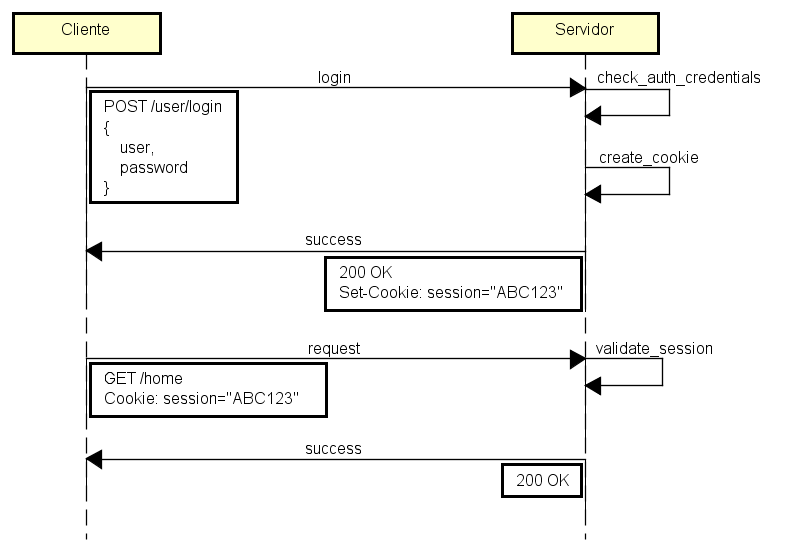
\includegraphics[width=.8\textwidth]{Session-Based Authentication.png}
  \caption{Exemplo de Autenticação baseada em sessão}
  \label{fig:sessionAuth}
\end{figure}